
%%
%% Template chap2.tex
%%

\chapter{Experiments}
\label{cha:results}

\section{Preparation of Datasets}
\label{sec:why2}


\begin{figure}[tbp]
	\centering
	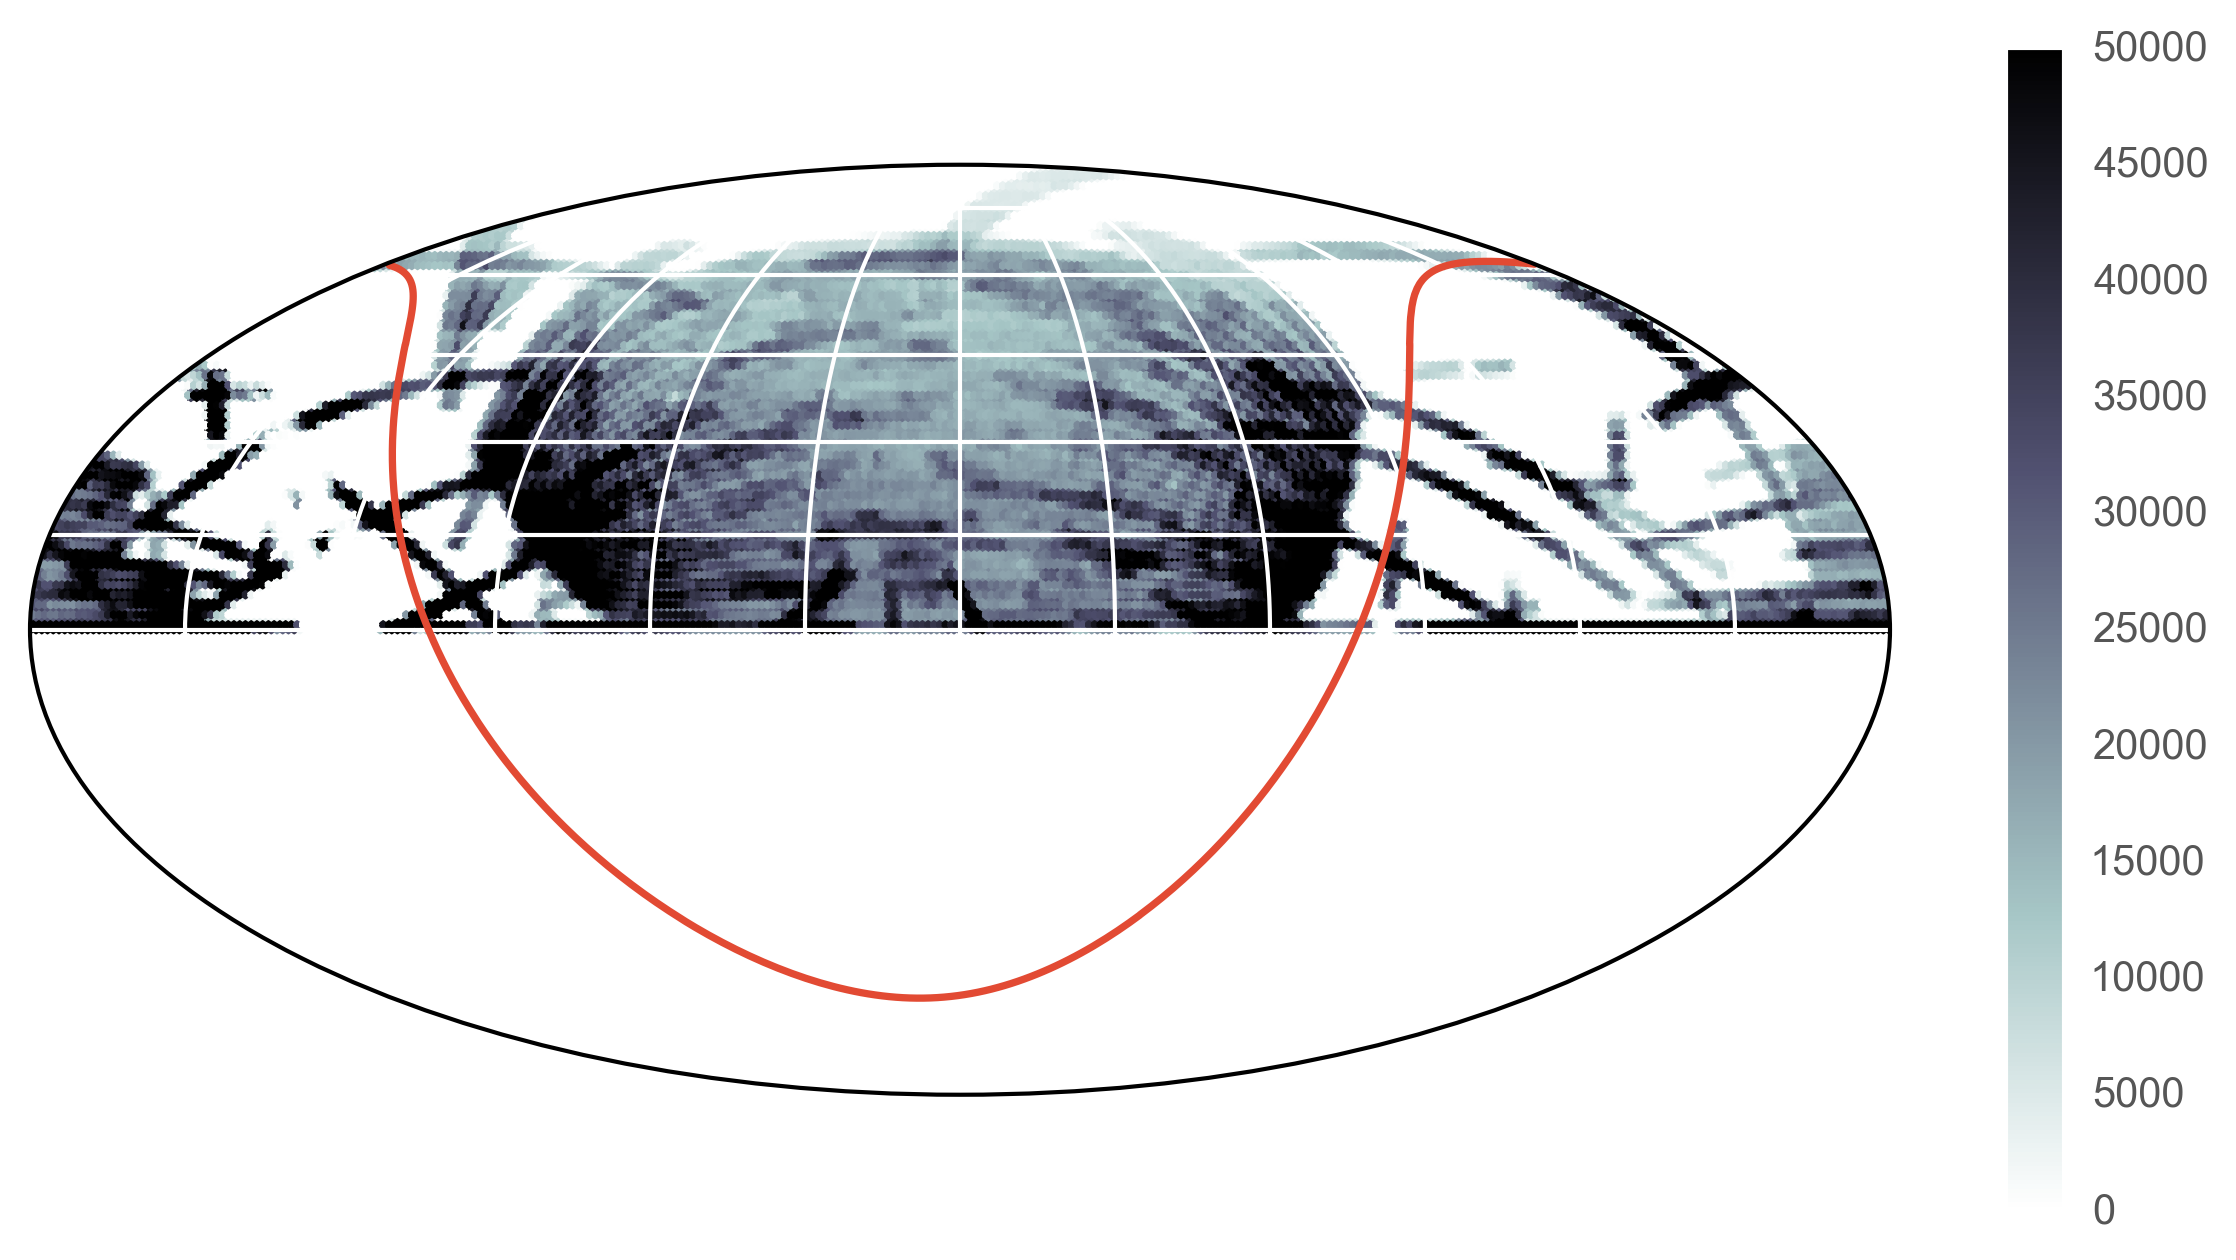
\includegraphics[width=0.75\textwidth]{figures/map_prediction_forest_all}
	\caption{Coverage of the SDSS}
	\label{fig:coverage}
\end{figure}

\begin{figure}[tbp]
	\centering
	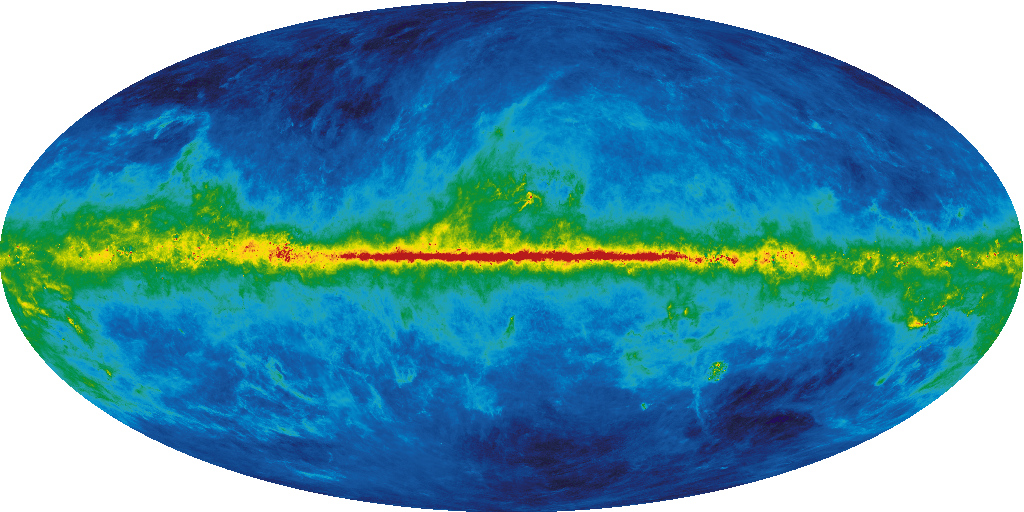
\includegraphics[width=0.5\textwidth]{figures/galactic_reddening_ebv_map_sfd98}
	\caption{Galactic Reddening $E(B-V)$ Map (SFD98 Correction Set)}
	\label{fig:reddining}
\end{figure}




\begin{figure}[p]
	\centering
	\begin{subfigure}{\textwidth}
		\centering
		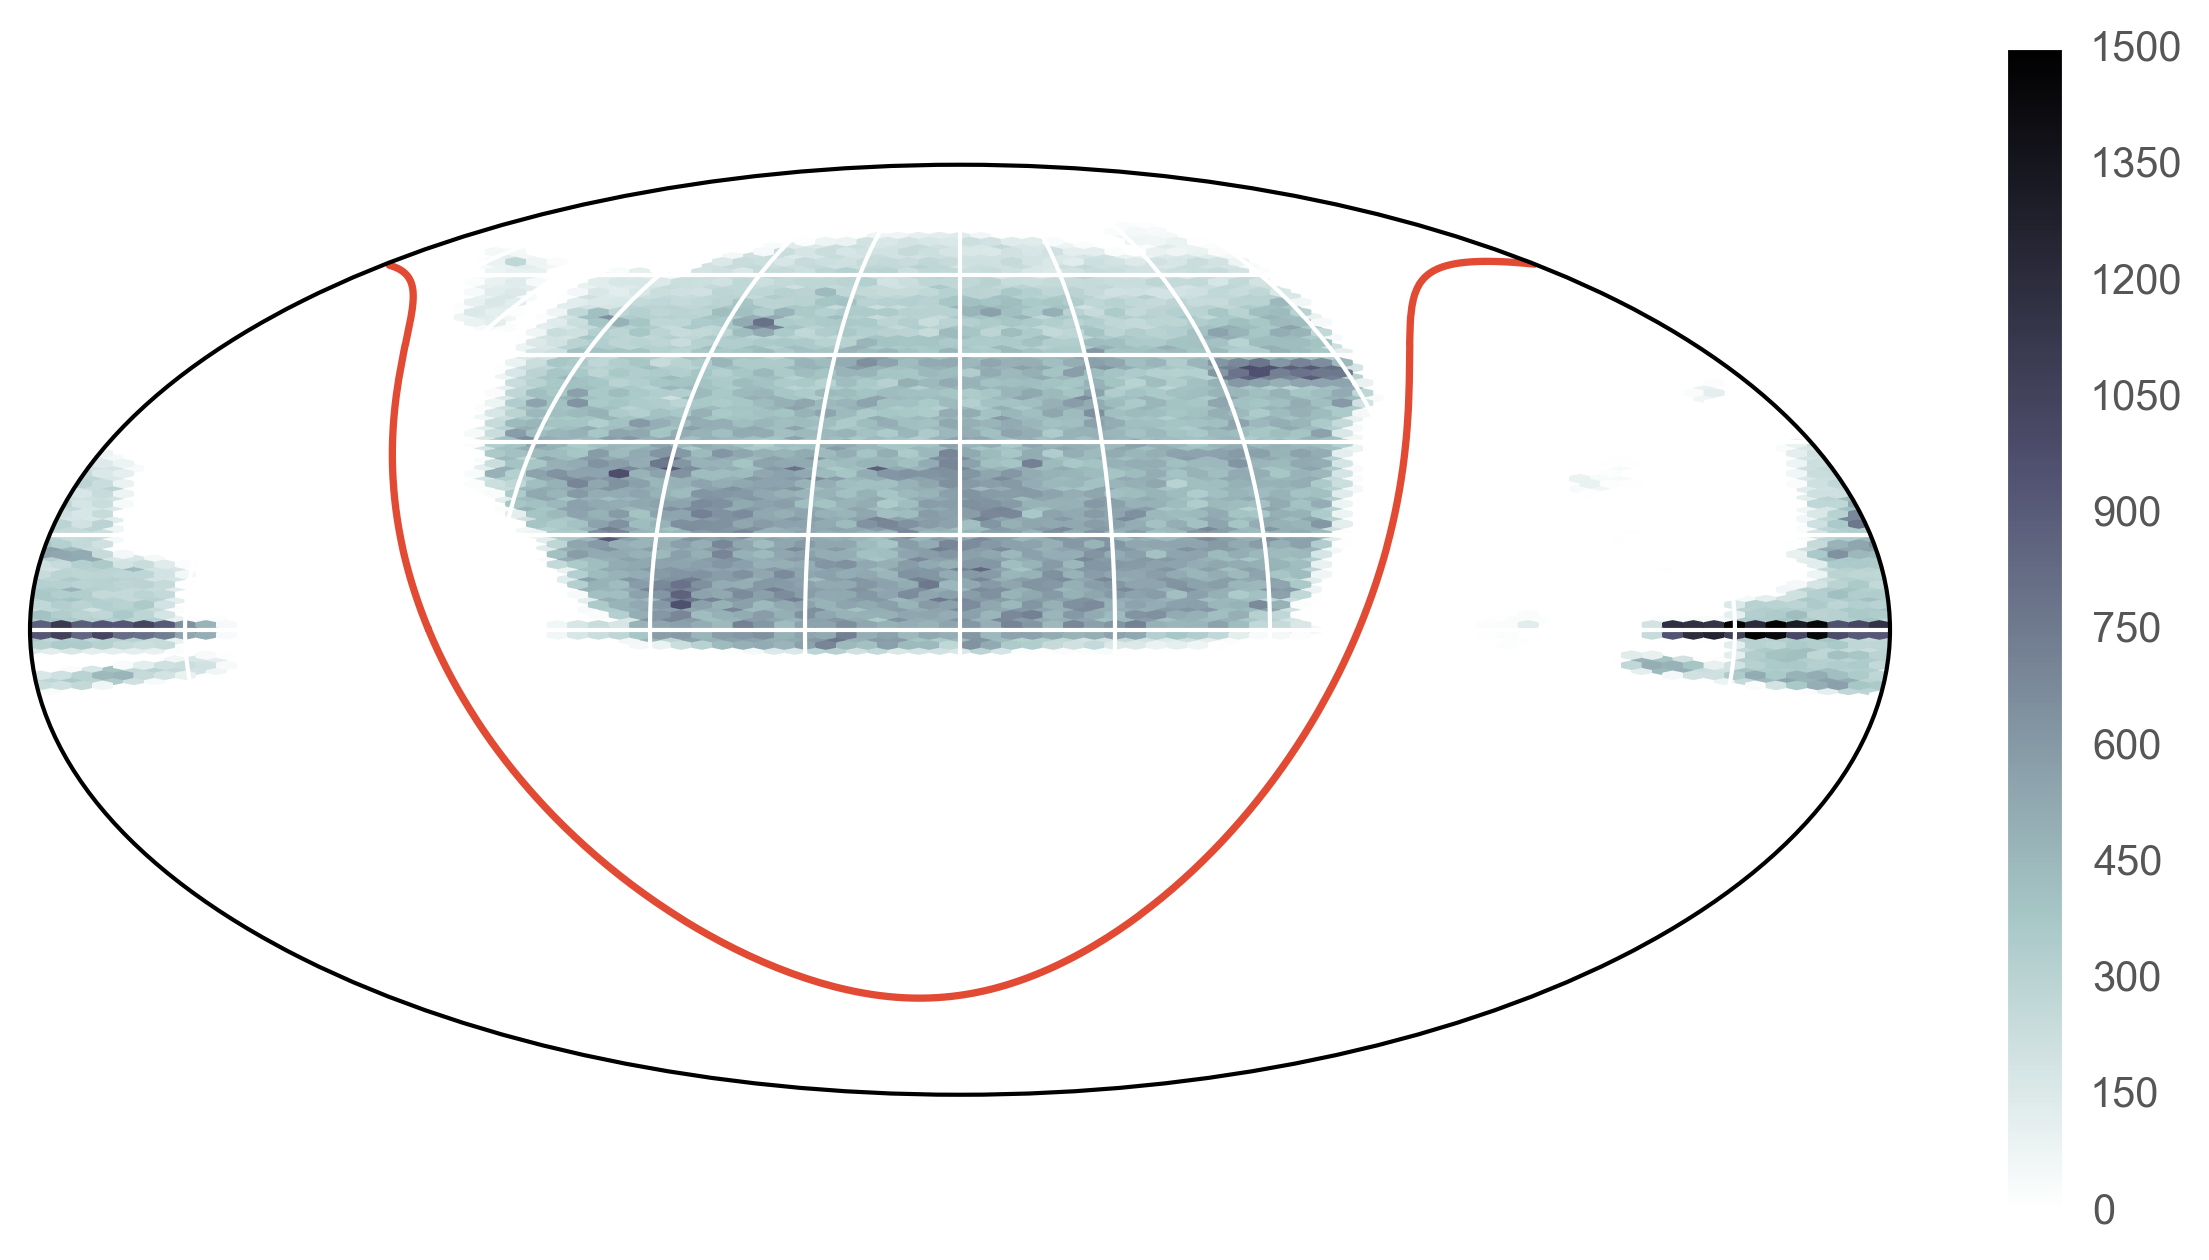
\includegraphics[width=0.75\textwidth]{figures/map_train_galaxies}
		\caption{Distribution of galaxies.}
		\label{fig:orbit1}
	\end{subfigure}\\
	\begin{subfigure}{\textwidth}
		\centering
		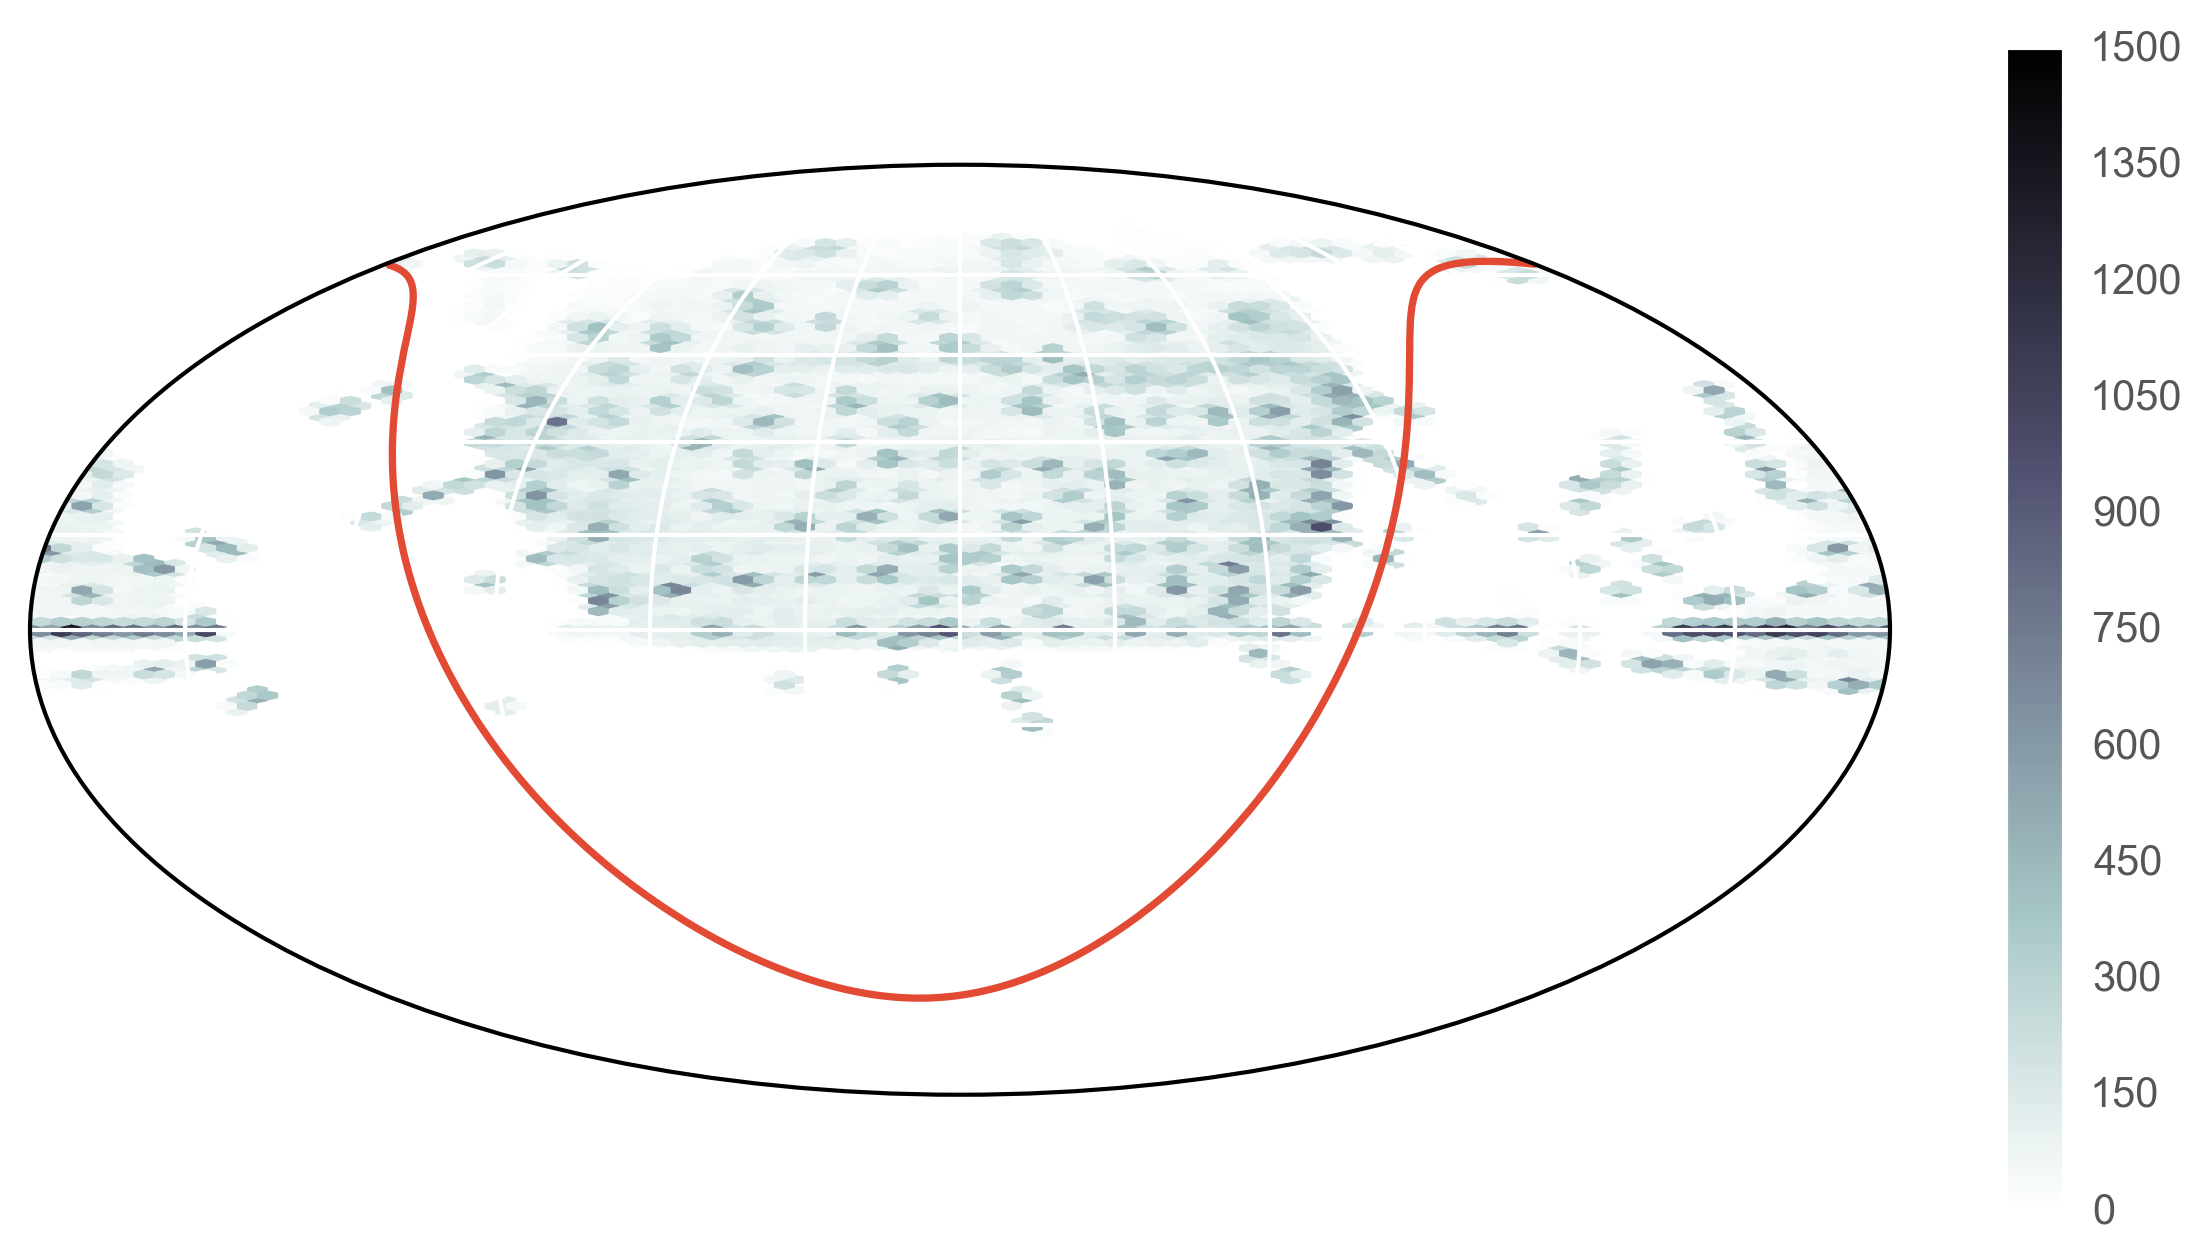
\includegraphics[width=0.75\linewidth]{figures/map_train_stars}
		\caption{Distribution of stars.}
		\label{fig:orbit2}
	\end{subfigure}
	\begin{subfigure}{\textwidth}
		\centering
		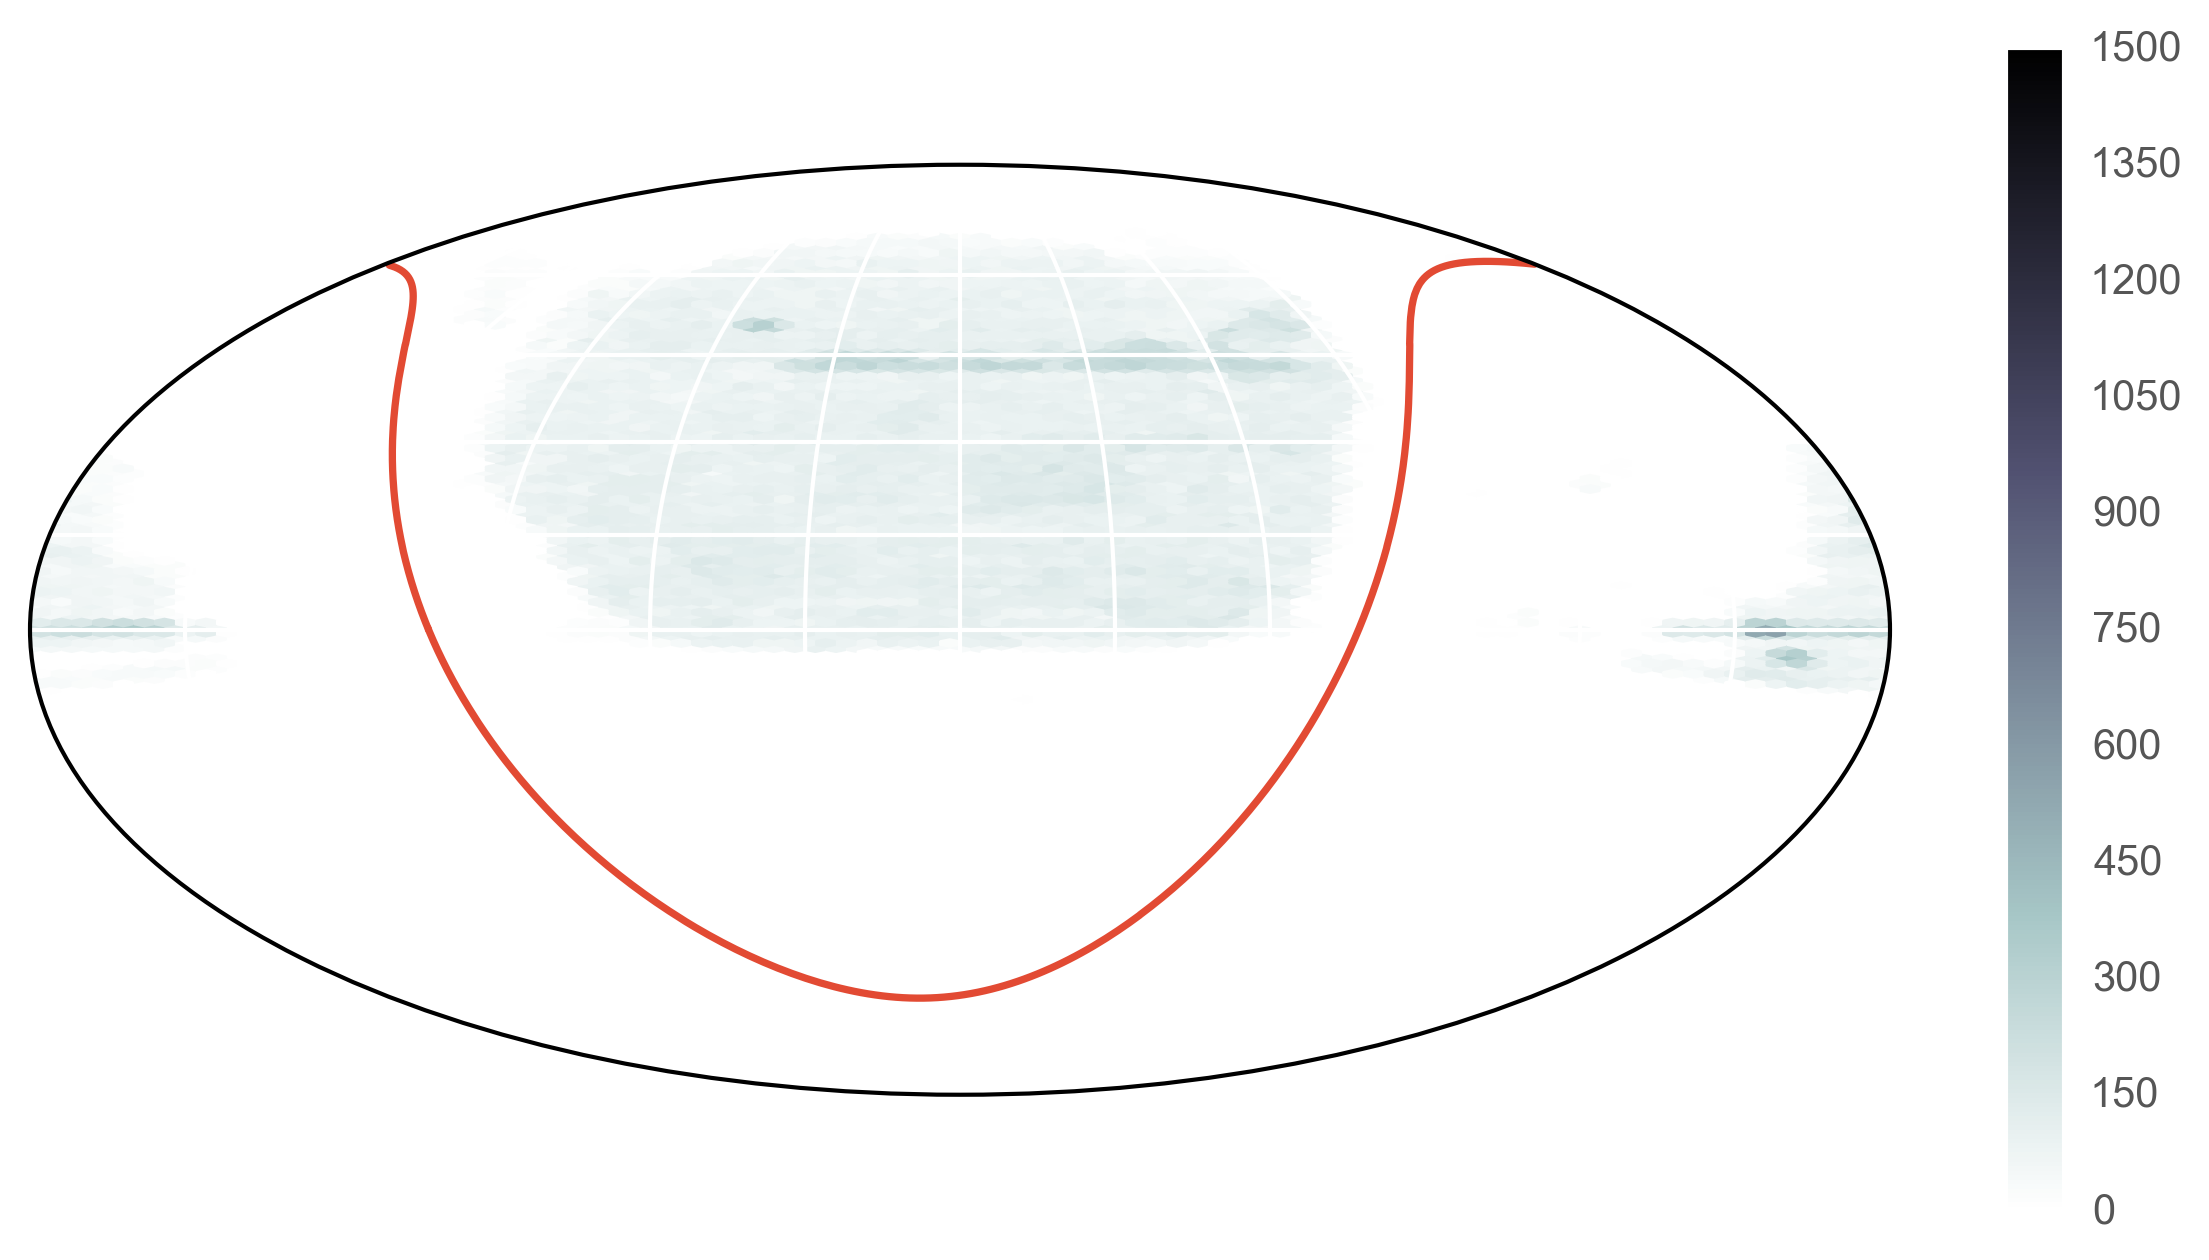
\includegraphics[width=0.75\linewidth]{figures/map_train_quasars}
		\caption{Distribution of quasars.}
		\label{fig:orbit3}
	\end{subfigure}
	\caption{Distribution of the classes in the SDSS training set.}
	\label{fig:orbit}
\end{figure}


\subsection{Feature Selection}

\section{Experimental Set-up}
\label{sec:what2}


\section{Results}
\label{sec:what}

\subsection{Class Proportion Estimation}

\begin{figure}[p]
	\centering
	\begin{subfigure}{\textwidth}
		\centering
		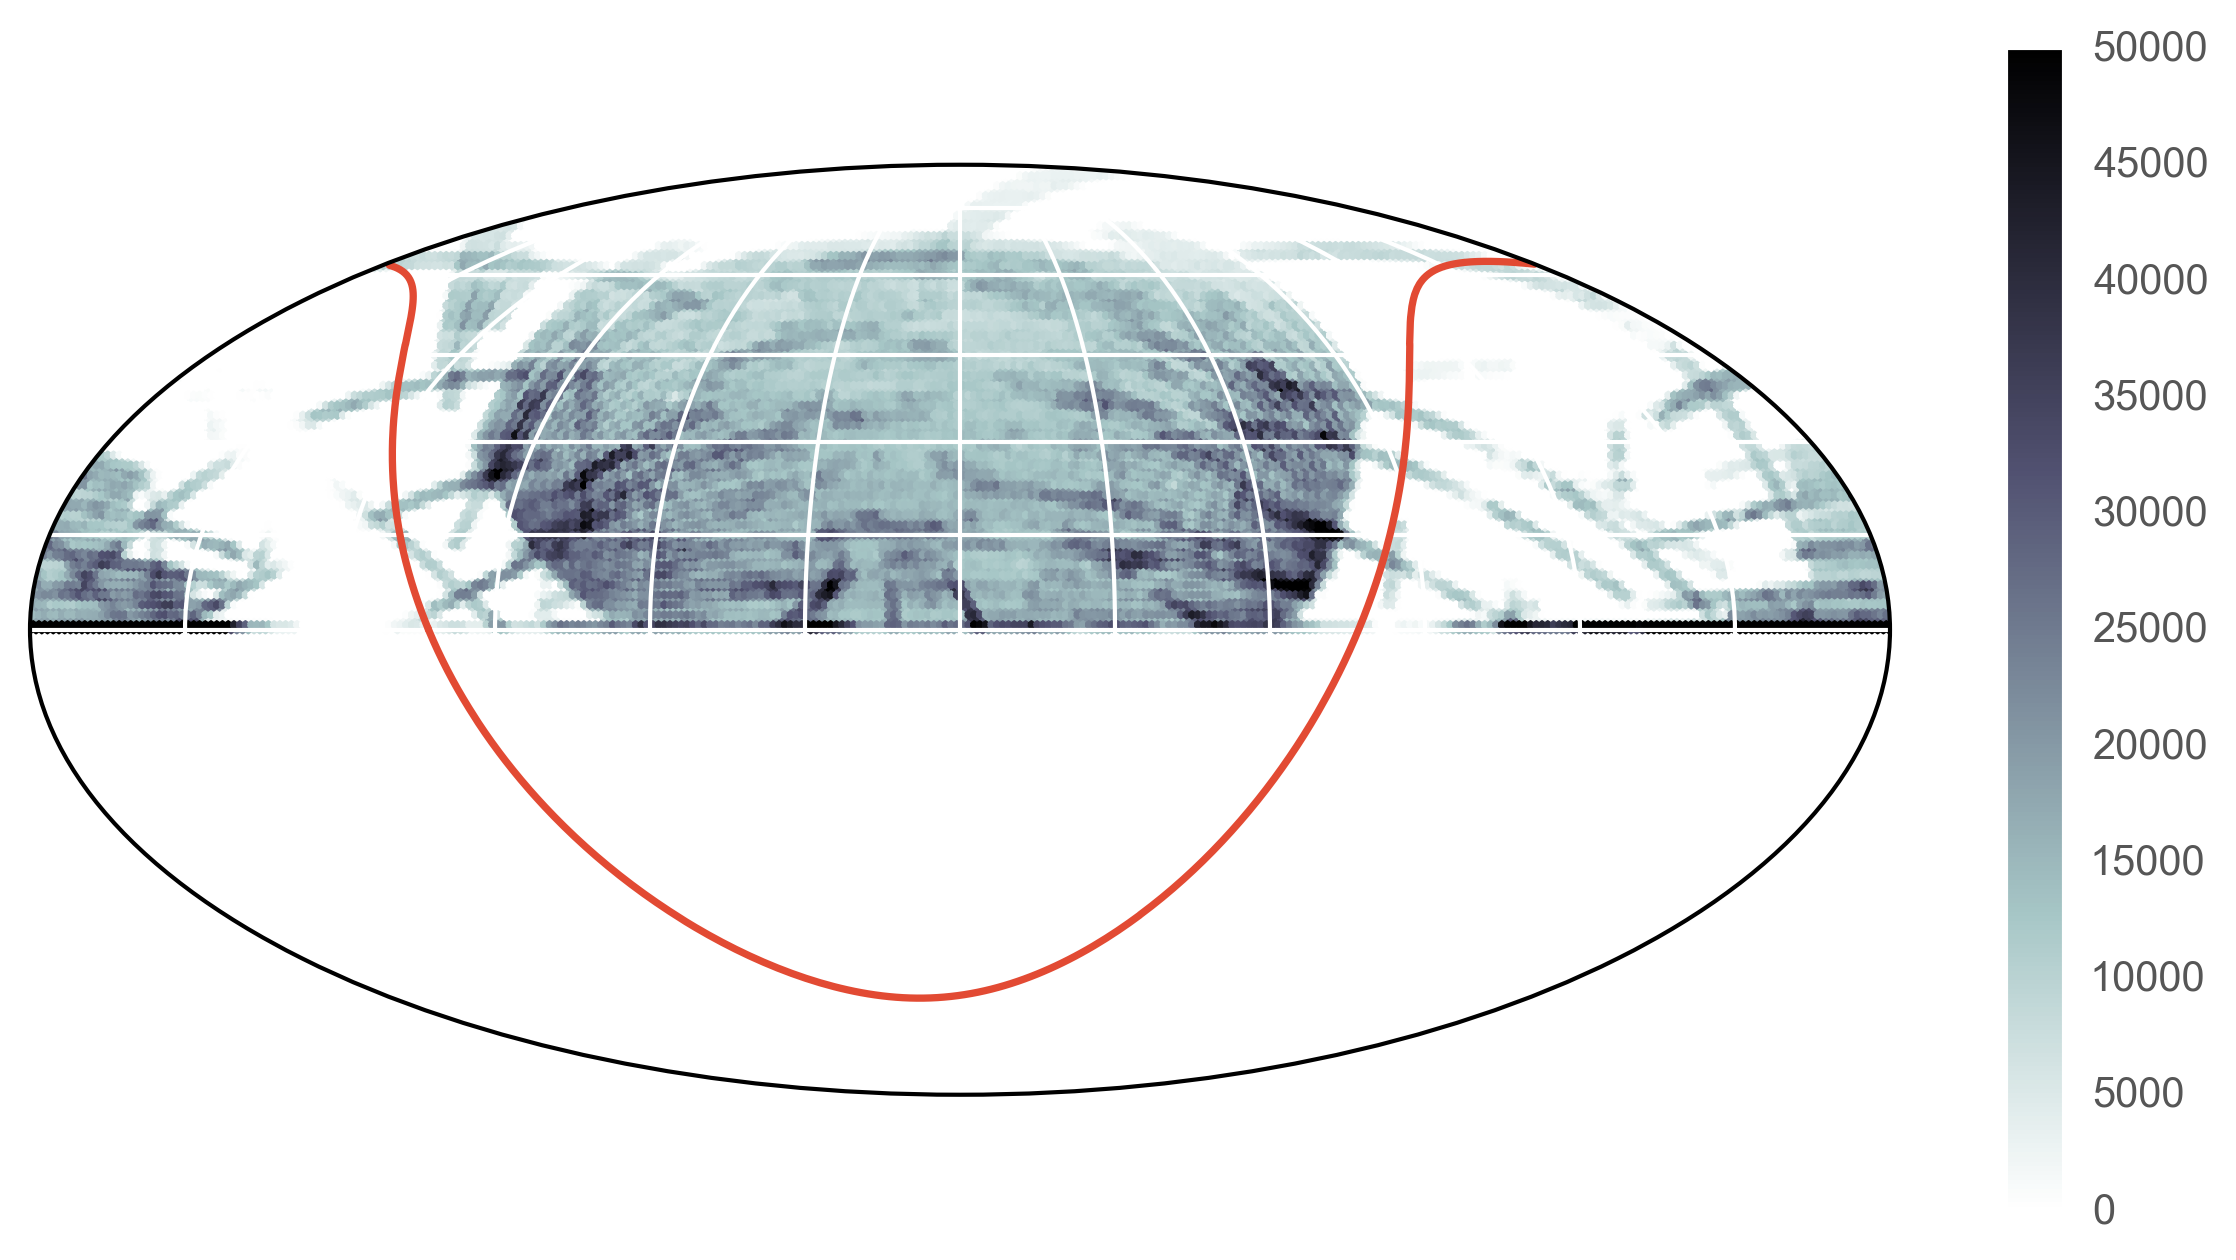
\includegraphics[width=0.75\textwidth]{figures/map_prediction_forest_galaxies}
		\caption{Distribution of galaxies.}
		\label{fig:random1}
	\end{subfigure}\\
	\begin{subfigure}{\textwidth}
		\centering
		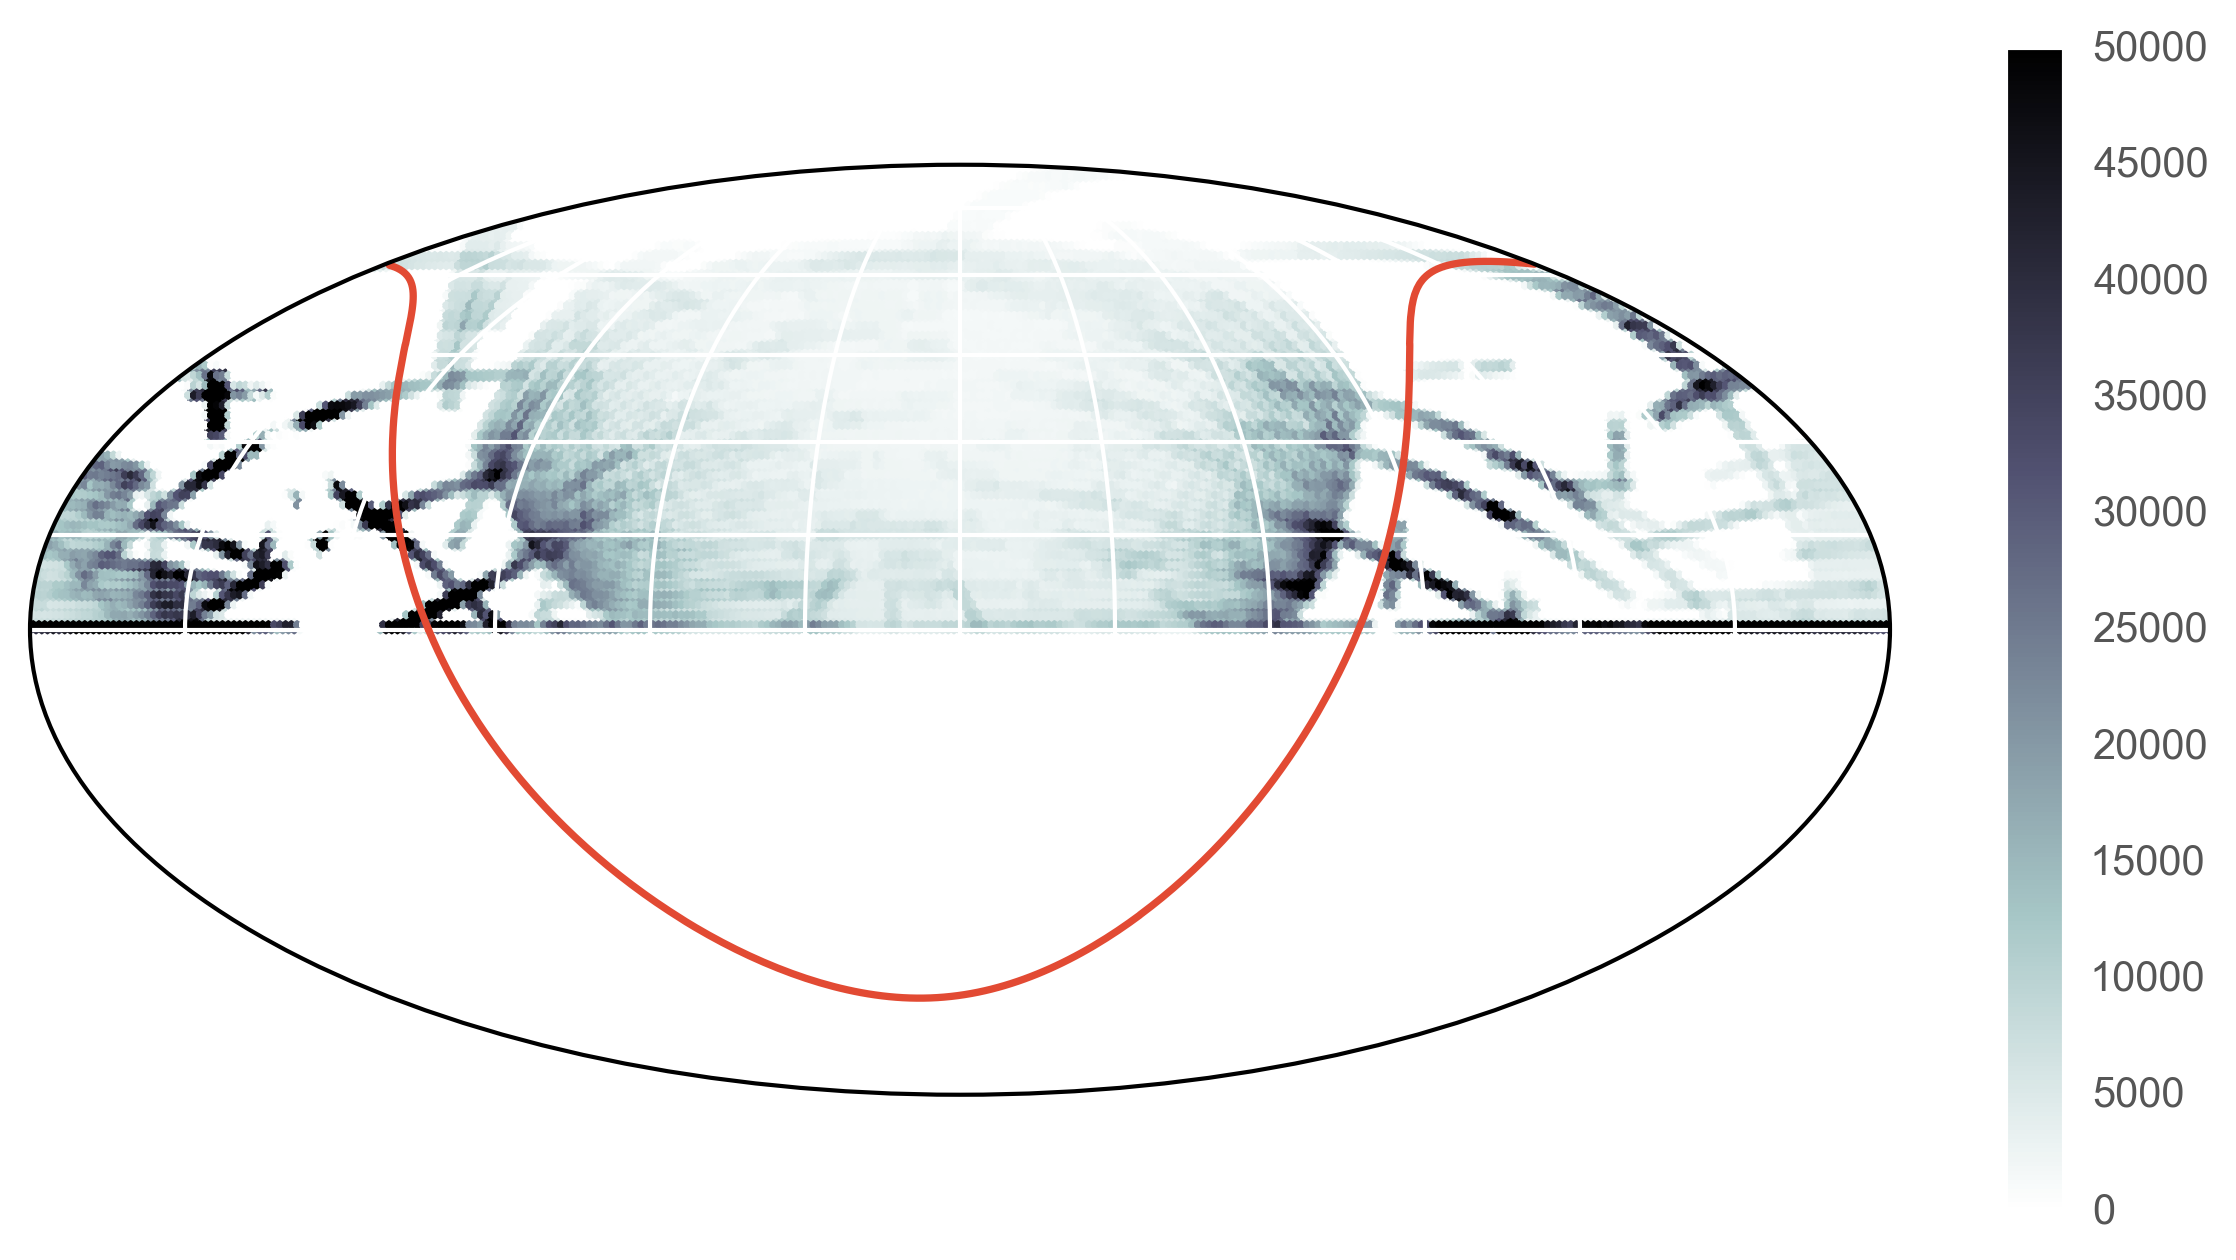
\includegraphics[width=0.75\linewidth]{figures/map_prediction_forest_stars}
		\caption{Distribution of stars.}
		\label{fig:random2}
	\end{subfigure}
	\begin{subfigure}{\textwidth}
		\centering
		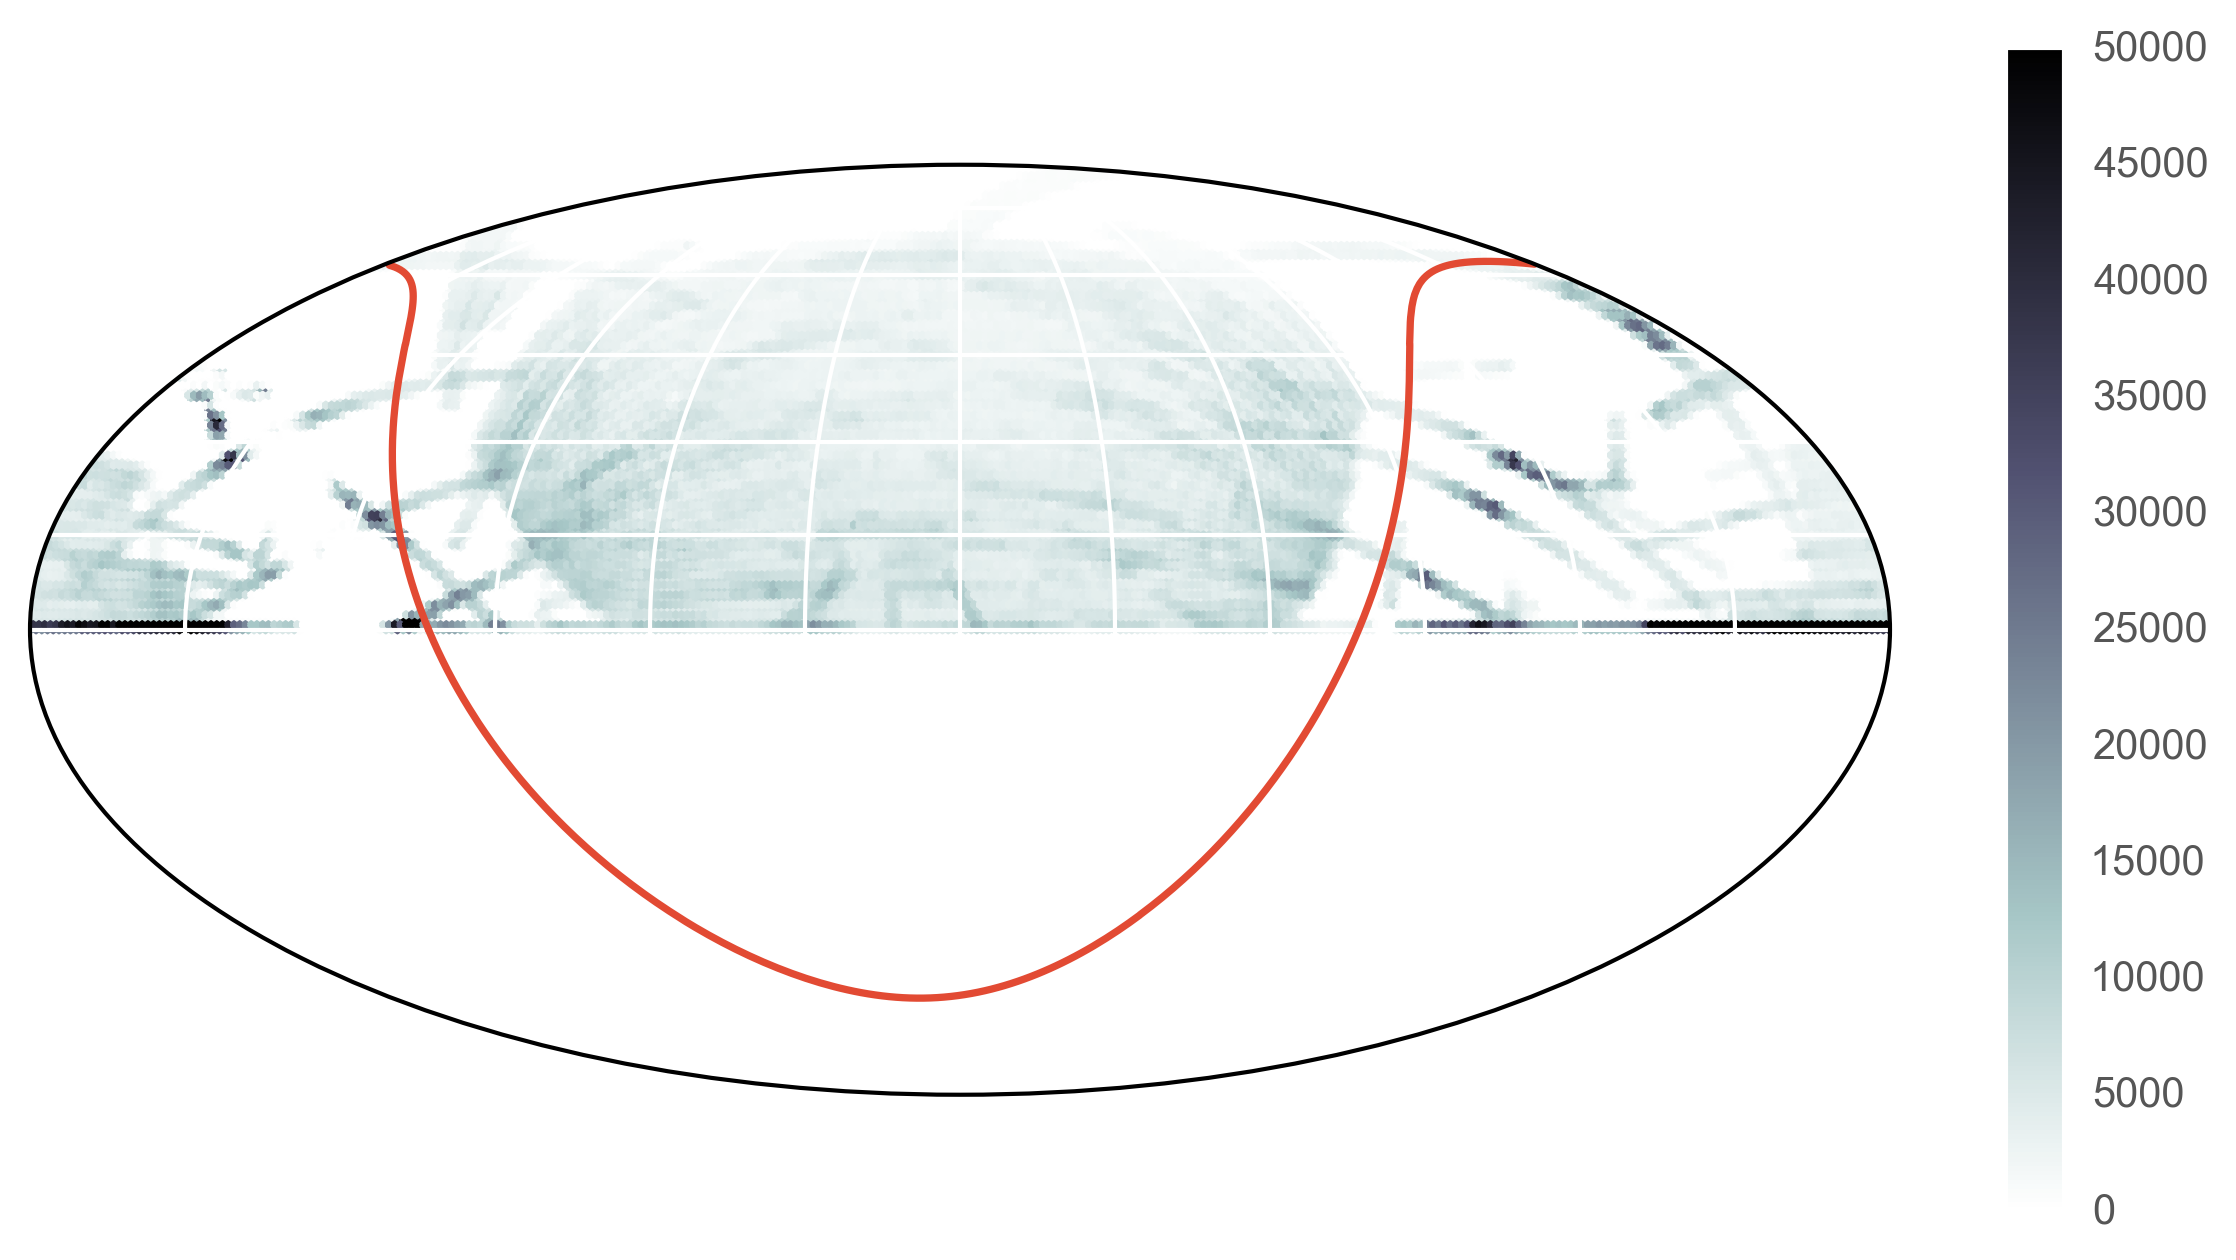
\includegraphics[width=0.75\linewidth]{figures/map_prediction_forest_quasars}
		\caption{Distribution of quasars.}
		\label{fig:random3}
	\end{subfigure}
	\caption{Map of predicted labels using random forest.}
	\label{fig:random}
\end{figure}


\begin{figure}[tbp]
	\centering
	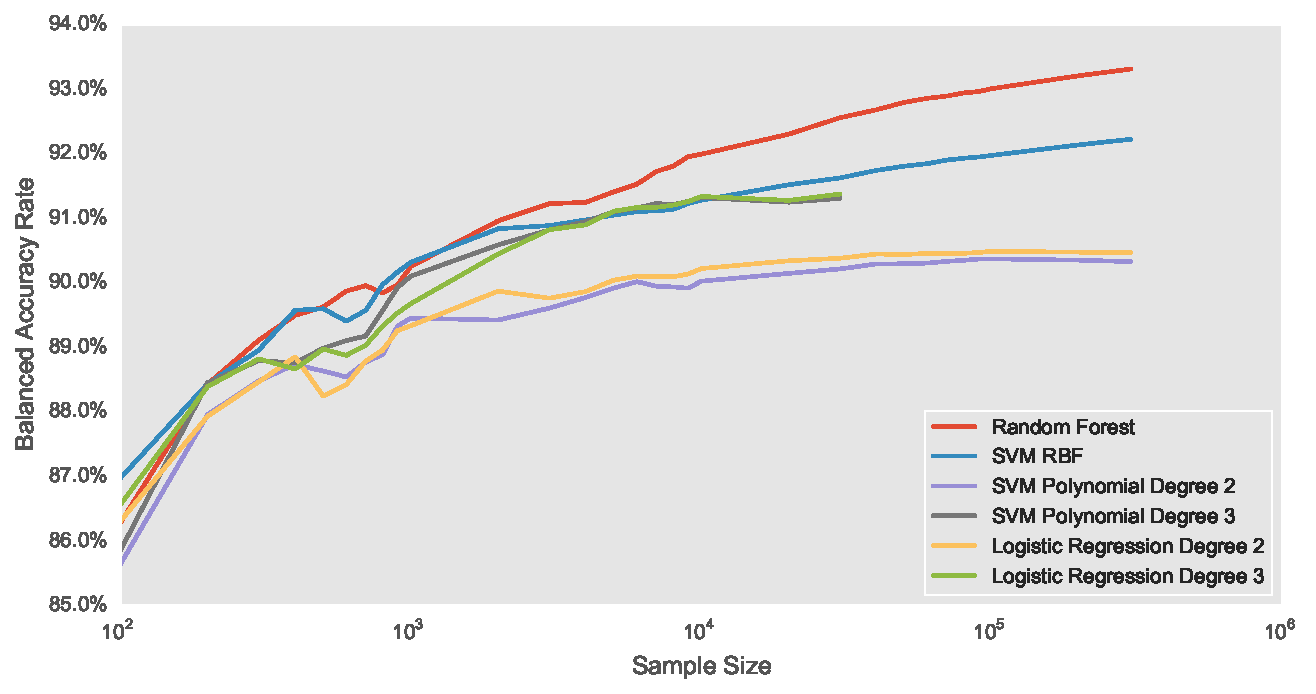
\includegraphics[width=\textwidth]{figures/learning_curves}
	\caption{Learning curves with random sampling.}
	\label{fig:learning}
\end{figure}



\section{Active Learning Results}
\label{sec:results1}

\section{Some More Results}
\label{sec:results2}

%%% Local Variables: 
%%% mode: latex
%%% TeX-master: "thesis"
%%% End: 
